\chapter{Soils: Connecting the Atmosphere, Lithosphere and Biosphere}\label{ch:soils}
\chapterauthor {Wilfrido Batista and Israel Teru\footnote{Statement of Contributions: Wilfrido Bautista wrote the introduction to soils, carbon pollution, and agriculture (above ground carbon sequestration. }}

\section{Soils as a Living Resource}

\subsection{SE Asia's Tropical Forests and Soils}

Southeast Asia lies right on the equator. The equator is home to much of Asia's tropical forests thanks to its relatively intense moisture and warmth. Anyone who visits these tropical forests will notice the cramped and dense canopy level, known for being evergreen and semi-deciduous (losing leaves for a relatively short amount of time, if at all) \citep{lieth2012tropical}. At low latitudes and with heat, the growing season in tropical forests is long and the rates of decomposition and nutrient recycling are speedy. While across all ecosystems, on average, 69\% of the carbon is stored in the soil and 31\% in living biomass, these accelerated processes stimulate an allocation of is about equal in parts in the tropics \citep{dixon1994carbon}. In this respect, deforestation in the tropics is noticeably more harmful than elsewhere.


\subsection{A Resource in Peril}

Tropical soils in Southeast Asia are some of the fastest deteriorating soils in the world. The deterioration is the result of anthropogenic disturbances, like the burning of vegetation, and its impact is ultimately determined by the existing development patterns-the pedogenesis- of the soil. Thus, as we determine ways to mitigate soil degradation, we must learn about both human-caused assaults and the given environmental backdrop of Southeast Asia. [Proposed thesis: In assesssing these two factors, we learn that hydrology, the movement of water in relation to land, is arguably the most important force in shaping soils in Southeast Asia. The region is enveloped by both the Indian and Pacific Oceans, impacted by monsoonal seasons, and contains roaring rivers like the Mekong.] 

Ever since the 1970s, the tropics overtook the temperate zones as the fastest cleared forests in the world, and since the 1990s have constituted almost all net forest clearance \citep{houghton1996land}. This is inextricably tied to carbon. Thanks to the aforementioned characteristics, tropical forests play a key role as a global carbon sink, meaning they can hold large stocks of carbon. In fact, they account for 37\% of the world's terrestrial carbon pool. This is especially crucial in the face of rapid industrialization and carbon pollution in Southeast Asia. In the past two decades, carbon emissions in the region have risen the fastest at a rate of approximately 5\% per year, and this has been accomplished with deforestation and consequent land use change \citep{dixon1994carbon}. In the next few sections, we will focus on building a knowledge bank on soils. We will then develop on the connections to carbon, and offer the reader new insights on Southeast Asia all along.

\subsection{Soil Ecosystem Services}

Soil is a resource that is non renewable and essential to life on Earth. Soil helps sustain many of the natural processes that happen on the Earth from water quality, land use, and vegetation security. 

When looking at the human production benefits for soil it literally grows the food we eat, adds fiber to paper and clothing, foundation for the roads and buildings humans make. Without soil the world as we know it would literally crumble to pieces and all chaos would ensue from the perspective of an natural scientist. Witnessing soils' natural attributes of mitigating pollutants and excess water, groundwater recharge, cycling of nutrients, and habitat for microorganism and biota. The vitality of soil is ever prevalent in the everyday lives we walk through.

\subsection{Soil Definitions}

The definition of soil by the Natural Resource Conservation Service (NRCS) touches upon its physical definition, natural body comprised of soils (minerals and organic matter), liquid, and gases that occurs on the land surface, occupies space and is characterized by one or both of the following: horizons, or layers, that are distinguishable from the initial material as a result of additions, losses, transfers, and transformation of energy and matter or the ability to support rooted plants in a natural environment \citep{baillie2001soil}. Other definition for soils is in environmental genetics terms is, the unconsolidated mineral or organic matter on the surface of the Earth that has been subject to and shows effects of genetic and environmental factors of: climate (including water and temperature effects), and macro- and micro organism, conditioned by relief, acting on parent material over a period of time. A product-soil differs from the material from which is derived in many physical, chemical, biological, and morphological properties and characteristics. 

\subsection{Soil Development: 4 Processes}

Four basic processes determine soil development: 

\begin{description}
	\item[Additions] is the concept of different elements and material adding to the already existing soil in the region. The materials are added to the soil through decomposing vegetation and organism or new mineral materials.  Natural elements that fall onto soil we see are water and dust added minerals. Organic particles we see is added by organic matter adding nutrients. Human influences of addition that we see in soil is fertilizer. 

\item[Losses] through the evaporation of water. When precipitation occurs we see soil particles wash away in the storm. The organic matter in the soil can erod breaking down into carbon dioxide.  Harvetation from the soil is other factor that occurs many times leading to poor soil conditions if excessive. We see physical/chemical of soil shifts leading to lost of many natural material within. 

\item[Translocations] move soil material whether organic or mineral between soil profiles. Organism that can burrow down into the soil can move materials through the soil to their benefit. We can see translocation through change in coloration differences, texture, and structure.

\item[Transformation] we see in the soil when chemical or biological process of the soil occur. We see transformation with leaf decomposition into humus. In the soil we can also see hard rock through weathering process turns into soft clay. Reduced Iron (Fe+2) in soil can react to oxygen that causes rusting.

\end{description}

\section{Vertical Patterns as Product of Pedogenesis}

\subsection{Biotic and Abiotic Factors}

Soils are the product of biologic activity -- but their development depends on a range of influential factors. 

These factors include abiotic characteristics: climate, topography, parent material, and time. In many cases, the trajectory of how these characteristics influence the development of soil is via water. Water promotes weathering of minerals, and chemical and clay translocations. 
 
\subsection{Role of Water}

Water also promotes the biotic factors, i.e. organisms that live in or interact with soils. With more water, we tend to see more above ground biomass. Depending on the water content of the soils, organic carbon stored in the soil can vary to a high degree.  Thus, soils provide an important mechanism to store carbon in the biosphere.


But water does much more. Chemicals and clays are transported downward or upward in the soils.
 
%storing carbon - inorganic and organic - and supporting plants which remove carbon from the atmosphere. 

%Our aim, then, is to also study the the carbon pollution and sequestration of Southeast Asia. The carbon influx we know is off balance and the implications of this are not fully understood. In this chapter, we will first give the reader the tools to understand basic soil processes and what kind of elements affect soil development in a global context. 

%We will then introduce the region's soil composition from the lens of geologists and biologists and summarize some of the most recent research concerns in the region. We will then contextualize these issues in the discourse on carbon by describing both the carbon storage capabilities of the region as well as carbon pollution in the region. In transferring knowledge and skills to the reader, this chapter cannot cover all of the information about soils and carbon, but instead it will be rooted in case studies and research that have been conducted in the region. Readers will thus learn about Southeast Asia and how to analyze like scientists. 


\subsection{Soil Horizons versus Sediments}

As a result of the vertical structure of biological activity, e.g. above ground deposition of detritus from plants or root uptake or turnover, soils develop important vertical structure that can be identified visually. The soil layers are defined as distinct layers called horizons (See Box). %that vary depending on the topography of the terrain.

(Insert Picure and Minipage :-))

The top uppermost layer is the O horizon composed of organic matter. This top horizon can vary in abundance due to factors like erosion.  We see a great distinction in O horizon in forested habitats. Subclassification of the O horizon are seen broken into three categories called hemic (Oe), fibric (Oi), and Sapric (Oa). The hemic (Oe) is known for having decaying matter with an identifiable origin of decomposition. The Fabric matter is organic matter that much unidentifiable origin of more decomposed matter. The last subcategory is the Sapric (Oa) is completely decomposed matter with unidentifiable origins. 

The next layer the A horizon is composed of a mainly minerals forming at/below soil surfaces. We can see either the presence of organic matter in this horizon as well. And if the use of tillage (cropping preparation) has been done to the soil we can see accumulated organic matter. The A horizon and O horizon can both play part each other when if heavy cultivation occurs on the soil leading to O horizon organic material to be found in the A horizon. 

The E horizon, known as the eluvial horizon due to the its loss of clay, iron(Fe) or aluminum Al is most common mineral horizon in forest soils. The loss of these dark minerals is due a leaching of nutrient via root zone due to water movement through the soil horizons. This leads to lighter mineral color like quartz, silica, or other minerals being the most abundant in E horizon. The E horizon is seen as a lighter horizon compared to the other layers present due to this reason.

The B horizon is most commonly found below the O, A horizons and either below or above the E horizon. The B horizon receives the deposited dissolved material of clay, iron and aluminium oxide, organic matter of decay plant and animal matter, carbonates, gypsum, and leached silicates from other layers. The presence of the Fe and Al oxide give the B horizon its reddish dark color than other horizons. 

The C horizon is home to little soil influenced by weathering process. This leads to presence of more parent material which attribute to the the chemical and physical properties of soil. There is a clear transition in this horizon from soil to bedrock

The last horizon is the R horizon which consist of complete bedrock. In terms of depth into the soil where you can find R horizon it strictly depends geographic location, environmental conditions, and landscape position it can go as deep as 100 feet or a few centimeters from soil surface. Bedrock is a strong reinforced rock that has fallen to the soil properties of the terrain. The deeper the bedrock the more we see a characteristic of biochemical weathering. While newly weathered bedrock is known as saprolite/saprock 

\subsection{Weathering Processes that Shape Soil}

When looking at soil formation we need to take in account the different occurrences that can affect forever changing soils. The change of soil formation are largely determined by the weathering of rock. Rock can go through three different types of weathering. \textcolor{red}{[HELP, I only see three categories of weathering, what am I missing? Perhaps Biological weathering?]}

Physical weathering is the when an adequate amount of stressed is applied to rock to break it. The processes that help in this process of physically breaking rock are erosion, freeze- thaw cycles, bioturbation, the presence of cracks or gaps in soils. 

Chemical weathering deals with the changes in the chemical nature of rocks. This occurs with mineral structure, reactivity, surface area, and particle size. The occurrences normally happen when there is instability of primary minerals at the Earth's surface, which is driven by instability of minerals. There must be exposure to the environment for the weathering process to happen. When looking at primary minerals and secondary minerals the presence of secondary minerals that are based off primary minerals show there will be a significant amount of clay. The presence of clay shows evidence for weathering because it is proof there was a secondary elements. Chemical weather increases in warmer, humid climates, with water and oxygen. We also see biological weathering with the microbial and plant root metabolism acid \citep{brady2007colloidal}. 

Chemical weathering processing can happen in four ways. Oxidation is one of the chemical processes that can happen in soil that involves high oxygen supply leading to an elemental lose of electrons. Reduction is the gaining of electrons and happens in environments where oxygen is decreasing. Hydration is the presence of water molecules in the mineral structure. Hydrolysis is hydrogen ions (water) presence in breaking down silicate structures (rock.)
 
\section {Soil Classification Schemes}

\subsection{USDA versus FAO versus other Classification Schemes}

Soil classification systems used by the United States of Agriculture (USDA) is the  Soil Taxonomy system \citep{soil2003keys}. The system is morphologically focused that uses quantitative and soil genesis to make soil groups \citep{buol1999oxisols}. The classification system is hierarchical with six levels that is 1) Order, 2) Suborder, 3) Great Group, 4) Subgroup, 5) Family, and 6) Series. There are 12 soil orders in the soil systems and each have differing characteristics (Table~\ref{}). 

Entisols are known for being the youngest formed soils in soil order. They normally include weak profile of soil layer development meaning horizon difference  aren't as a differentiable. Entisols can be found in use in agricultural spaces (plow layer), steep slopes with severe erosion, and  floodplains.  

Inceptisols soil orders are characterized for being young and having little to no soil profile development at all. We find them mostly alongside rivers and streams due to this.  

Both Entisols and Inceptisols have the potential at a later time to develop intricate soil horizons. The thing playing as a major influence in these soils is parental material unlike other soils likely influenced by climate and vegetation. 

Gelisols are considered young soil orders in terms of geologic time and are found in colder climates. The condition they are found in are permaforst and cryoturbation in Canada and Alaska \citep{soil2003keys}. 

Mollisols are prairie soil mainly found in midwestern United States where they dominate landscapes. They are known to be characterized for their high organic content, dark colors, steep A horizons. The category to be met for the A horizon is that it must be 8 inches deep and must be 50\% saturated. Alfisols can be found in midwestern America as well and are normally in deciduous forest habitats. Alfisols are found in humid landscapes globally and have have E horizons.  The base saturation for these soils must be at least 35\%. 

Spodosols originate from parent material that is acidic in nature and areas of loamy/sandy content. We normally see spodols in forest vegetation like coniferous forest due to pine needles high acidity when decomposing. \citep{brady2007colloidal} We normally see the presence of a bright red horizon below a white E horizon.

While these classification of soils is effective. We must be mindful that the data was created by the United States Department of Agriculture (USDA) in the 1970s. The implications of it in a global context may not cohesively translate and the way locals in native Southeast Asian countries classify things could greatly vary. A part of understanding soil is understanding the way locals interpret the data and be able to communicate across these boundaries for a better and new outlook.

\section{Contextualizing Soils in Southeast Asia}

As mentioned, soil is fundamental to the survival of humans: from plant growth, to water purification, to decomposers in the nutrient cycles, and even to bacteria that have been used for developing antibiotics that treat human disease \citep{asio2006morphology}. Soil degradation caused by physical and chemical occurences (like wind or loss of nutrients), are now widespread, putting tropical fauna and flora as well as humans who depend on agricultural productivity at risk. The National Action Plan of the Philippines, for instance, has identified soil degradation as a major threat to soil productivity and water retention (The Updated Philippine National Action Plan to Combat Desertification,Land Degradation and Drought, 2010). Soil degradation was coined in 1888 to describe natural soil changes, but according to the Global Assessment of of Soil Degradation has since come to define human-induced disruption because of the aforementioned urgent crises (UNEP, 1992). Let us dive into the scientific history of soils in Southeast Asia so that we can better illustrate the context with which are dealing. [as part of thesis: As we walk through this history, we will demonstrate the impact of water, as molded by natural and anthropogenic processes, on the soil.]

\subsection{Geology and Soil Types}

The soils of Southeast Asia, particularly of islands in the region, are known to be generally much younger than those in Africa and the Americas \citep{juo2003tropical}. Much of the land rose from the oceans during the recent Cenozoic Era, which only spans the past 65 million years since the extinction of non-avian dinosaurs \citep{hall2002cenozoic}. 

The Quaternary period, the current period in the Era, brought a regime of monsoonal weather and limestones \citep{verstappen1997effect}, which humans have been exploiting for its initial crop productivity against acidic soils and its accessibility in low elevation \citep{asio2006morphology}. It is important to note that less pedological research (research on soils) has been conducted in Southeast Asia compared with geologically older regions, making the information presented here that much more relevant. 

In terms of soil types, Southeast Asia is an anomaly. While the Ferrasol group is the most common in the Amazon and Congo Basin, Southeast Asia is dominated by the Acrisols group \citep{kyuma1966major} -- the group covers 51\% of Southeast Asia. 

Acrisols can be found in a wide range of elevations, and they are generally confined to areas without a marked dry season. They formed on acidic to basic parent material, and in general they are relatively poor in nutrients and are susceptible to erosion. Ferrasols are also found in a wide range of elevations. They are fossil formations interacting with today's climate ranging from semi-hot equatorial to monsoon hot tropical. 

A lot of information about soils, particularly in developing nations, was consolidated through a two-decade global survey conducted by the Food and Agricultural Organization of the United Nations (FAO), UNESCO, and the International Society of Soil Science \citep{dudal2005soils}. Hence, most of the information presented here is extracted from the FAO-UNESCO Soil Map of the World Volume IX on Southeast Asia. Tables 1 and 2 present data about some of the subcategories of Acrisols and Ferrasols. These subcategories are chosen with a focus on mainland southeast Asia in mind as can be seen in Figure \ref{fig:mainlandsoils}.

Exercise 1: Find the document from the FAO-UNESCO Soil Map of the World Volume IX on Southeast Asia and add a soil subcategory to the tables below.

\begin{table}
  \caption{The data captures the characteristics of Acrisol subcategories, including properties relevant for agriculture. Information consolidated from the FAO-UNESCO Soil Map of the World Volume IX.}
\begin{center}
  \begin{tabular}{ | p{3.5cm} | p{3.5cm} | p{3.5cm} | p{3.5cm} |}
    \hline
    \multicolumn{4}{|c|}{Acrisols} \\
    \hline
    Categories & Ferric & Gleyic & Humic \\ \hline
    Tropical Forest Type & lowland evergreen rain forest & dry deciduous forest & montane rain forest | generally on non-volcanic mountain slopes\\ \hline
    Acidity & Alkaline & Alkaline &  Alkaline \\ \hline
    Natural fertility level & Low & Low & Medium \\ \hline
    Organic Matter Content & Low & Low & High \\ \hline
    Water Drainage & Low & Low & High \\ \hline
    Other Limiting Factors & iron concretions & &\\ \hline
    Agricultural Interference & requires heavy applications of phosphate, potassium and nitrogen fertilizers & requires irrigation syste for continuous water input & soil management to reduce erosion\\ \hline
    Suitable Crops & Rubber & rice & tea, upland rice, groundnuts, maize \\ \hline
    Other Comments & & dries quickly & slopes make erosion a hazard if deforested/exposed\\ 
    \hline
    \end{tabular}
		\end{center}
\end{table}
 
\begin{table}
\begin{center}   
    \begin{tabular}{ | p{5cm} | p{3cm} | p{3cm} | p{3cm} |}
    \hline
    \multicolumn{4}{|c|}{Ferrasols} \\
    \hline
    Categories & Humic & Rhodic & Xantic \\ \hline
    Tropical Forest Type & natural montane evergreen rain forest - developed from volcanic deposits & evergreen rain forest - developed on ancient basalt (type of volcanic rock) & poor evergreen rain forest\\ \hline
    Acidity & Neutral & Basic-Neutral & Neutral-Acidic \\ \hline
    Natural fertility level & Low & Low & Low \\ \hline
    Organic Matter Content & Med-High & Med & Low-Med \\ \hline
    Water Drainage & High & High & High \\ \hline
    Other Limiting Factors & often found with a layer of ironstone concretions within rooting zone & & hard layer of iron concretions\\ \hline
    Agricultural Interference & typically not used for agriculture & little phosphate and nitrogen fertilizer & typically not used for agriculture\\ \hline
    Suitable Crops & none & rubber, coffee, fruit trees, tobacco, maize & \\ \hline
    Other Comments & used for timber if anything & crumb top layer makes it resistant to erosion & should be reserved as natural forest\\ 
    \hline
    \end{tabular}
    \caption{Table 2. The data captures the characteristics of Ferrasol subcategories, including properties relevant for agriculture. Information consolidated from the FAO-UNESCO Soil Map of the World Volume IX.}
\end{center}
\end{table}

\begin{figure}
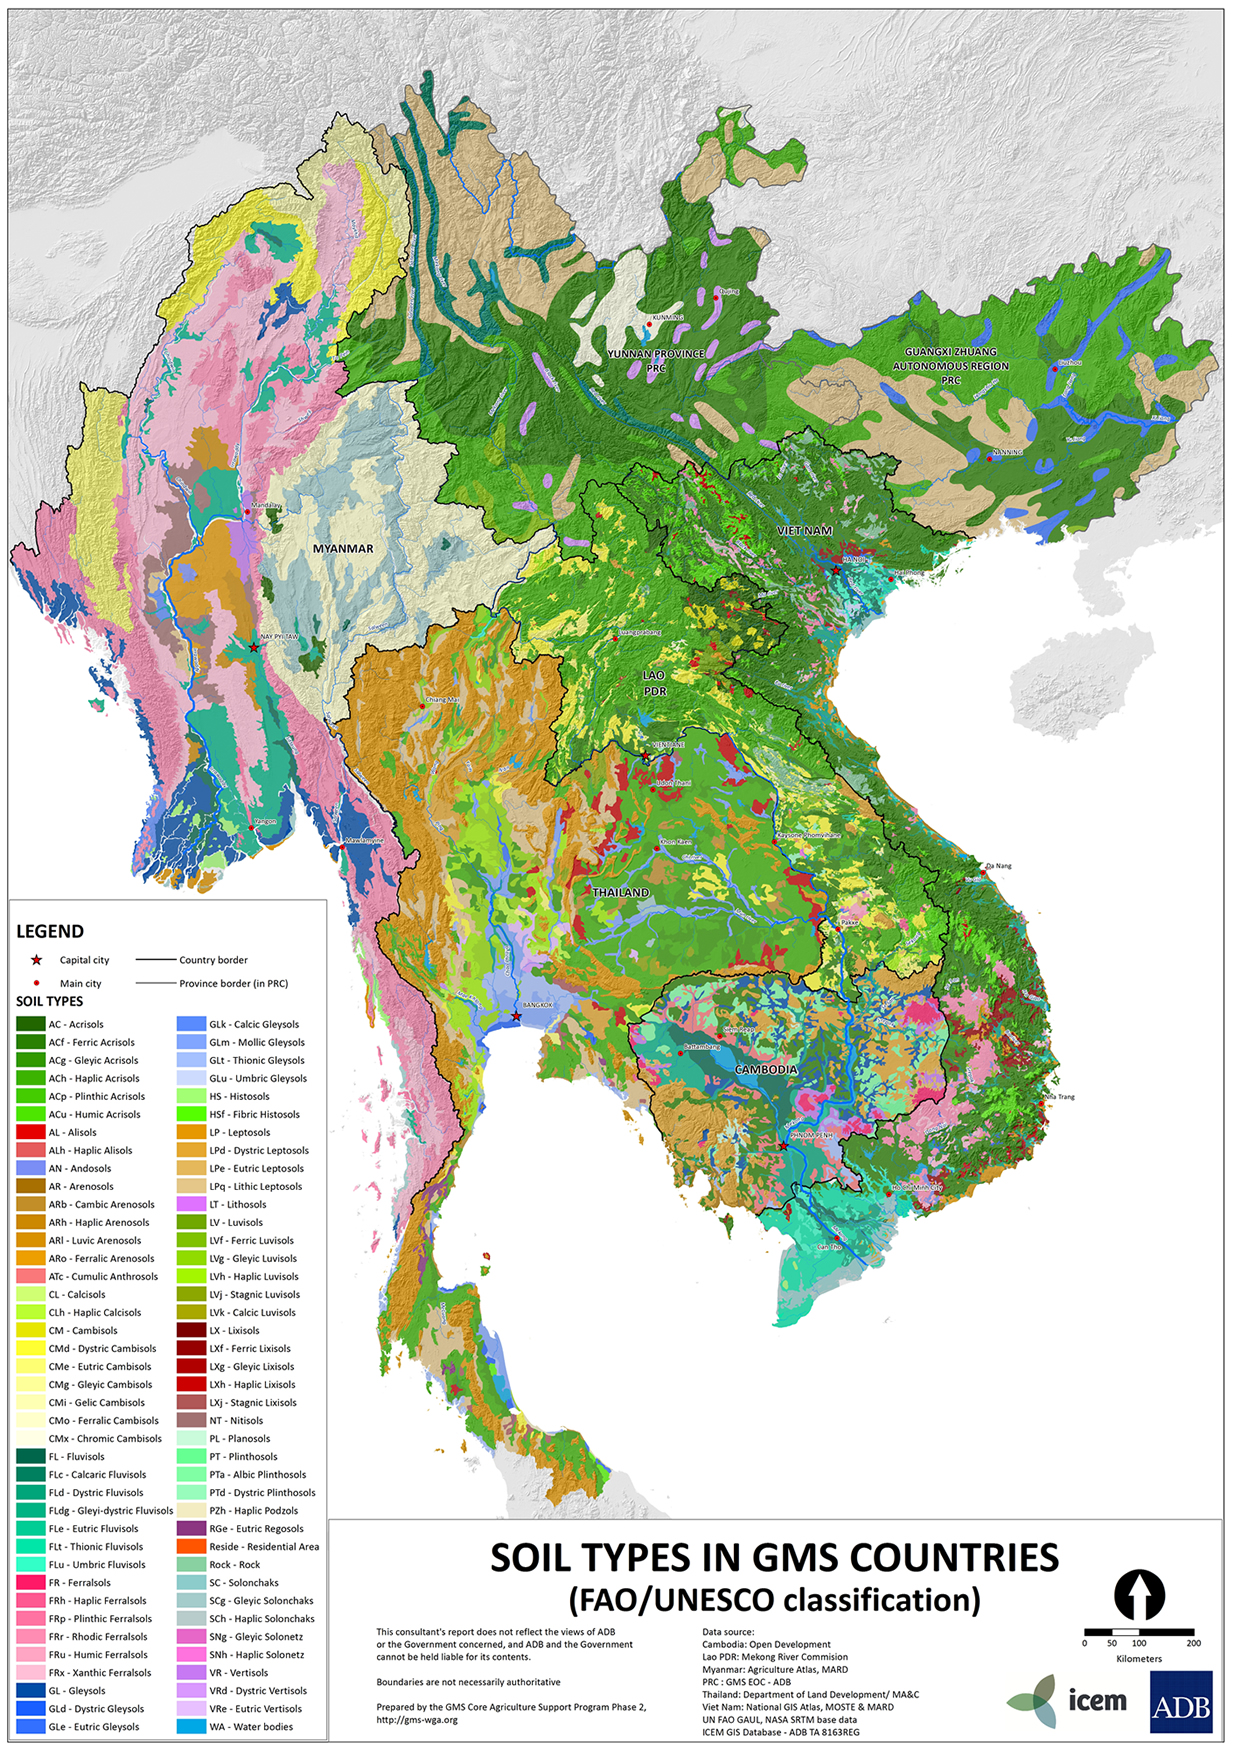
\includegraphics[width=\textwidth]{mainlandsoils}
\caption{Soil Types in GMS Countries}
\label{fig:mainlandsoils}
\end{figure}

\section{Human Impacts on Soils}

\subsection{Hydrology and Soil Erosion}

\textit{Horizontal and Vertical Interfaces} \newline
Soils act as key players in global interfaces which are both horizontal and vertical. They serve as the intersection of many scientific subjects -- take hydrology for instance. Hydrology relates water to land through vertical and horizontal interactions. It is important to study hydrology because we can learn and predict about relevant environmental conditions like time and scale of flooding, distribution of moisture in the soil which relates to the distribution of plants, chemical and sedimentary transmission from the built environment to rivers, and agricultural productivity \citep{chappell2010soil}. In 2001, Elsenbeer fostered the notion that subsurface water pathways in the tropics start with vertical flow in Ferralsol soil and transition to lateral flow in Acrisol soil \ref{fig:ferrasol and acrisol} \citep{elsenbeer2001hydrologic}. The study has been shown to have some inconsistencies, partly a result of the better definitions that exist for soil types today. It has been found that the proportion and type of clay in the soil can lend these types of soils a wide range of vertical and lateral properties. For example, Bukit Timah in Singapore is dominated by Acrisols with kaolinite, a type of clay, and has less than 10\% lateral flow \citep{chappell2005contrasting}. Hence, generalizations like Eisenbeer's should be questioned. One can now see how picking up on such nuances is crucial to scientists.


\begin{figure}
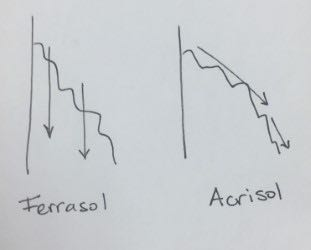
\includegraphics[width=\textwidth]{ferrasolacrisol}
\caption{Elsenbeer's Hypothesis on the Water Pathways in Ferrasols and Acrisols}
\label{fig:ferrasol and acrisol}
\end{figure}

Taking us back to the geologic timeline, quaternary soils are known to be generally unconsolidated, also holding many hydrological properties such as fluvial (river) deposition, marine inundation, slope wash and more \citep{chappell2007runoff}. Many of the sediments in Southeast Asia are loose, attributing soil permeability to regions like the Mekong Lowland of Cambodia and Central Plain of Thailand \citep{chiem1993geo}. This means that rainfall does not simply reach river by a lateral pathway over land, instead it can often times percolate before it reaches rivers. Aquifers, large areas of underground water characterized by porosity and ease of percolation, are found in these regions \citep{struckmeier2004groundwater}. \newline


\subsection{Soil Erosion}


Although Southeast Asia is one of the zones most vulnerable to climate change, not enough research has been conducted about its impact on soil erosion in the region. With climate change, rainfall can sporadically increase and turn more aggressive, leading to greater soil erosion \citep{chappell2007runoff}. There are a host of reasons that may be hypothesized: soil erosion can intensify as the canopy changes in response to variable moisture in the air and ground, as cover on the ground changes in response to variable decomposition rates, and as soil moisture changes in response to variable evapotranspiration rates (rates of evaporation from the soil to the atmosphere), and as land use changes in response to economic demands. In short, the implication of climate chage exacerbate the impact of rainfall on soil erosion. 

The effects of rainfall can be even worse in slopy areas. There has been special concern in watersheds shared between countries in Southeast Asia because these border zones generally require much-needed collaboration and data-sharing.\citep{giang2017spatial} In the aforemention paper, Giang and colleagues assessed the interaction between rainfall and soil erosion in the Laos-Vietnam transnational Upper Ca River Watershed (UCRW). The UCRW is an important site for agricultural cultivation, and its hilly topography makes it especially sensitive to acute rainfall. Evidently, there is an economic incentive to implement conservation practices in the region. The study found that spatial and temporal factors should be considered. First it was observed that much of the hill-slope erosion is found in the upstream and middle stream areas. Understandably, it was also found that sediment transport would occur mostly in the wet season when it is warmer and wetter. Therefore, to protect residents and cultivation, special attention should be paid in the months between August and October. 

To slow soil erosion, both institutional and individual measures should be applied. At the administrative levels, it should be understood that groundcover other than farming and normal anthropogenic use is necessary. Rehabilitation of the land is possible with reforestation, afforestation (foresting land at which tree cover has been absent for longer), terrace farming (farming on sloped planes with a series of flat planes), as well as check dams. At the domestic level, and just as importantly for the less hilly areas (such as downstream of the UCRW), farmers can learn and practice crop rotation, cover cropping, and mulching.

\subsection{Agriculture and the Soil}


As we have seen, agricultural soils can significantly alter the landscape. This can also be recognized in its impact on biodiversity. Southeast Asia is well-known for being a biodiversity hotspot, with many endemic species that rely on an established and robust food web system \citep{tripathi2012tropical}. We will use a study from Malaysia on the soil bacterial community, organisms which are much less researched and appreciated by the general public, as our kickstarter. 

Research on microbial communities around the world has been concerned with comparing their activities in forests versus agricultural lands. We ask: How do the two environments structure the accompanying bacterial communities?  What are the specific environmental factors that may explain these observable differences?

The Malaysia-based study found that, in general, the bacterial community composition was most influenced by the acidity of the soil, followed by total carbon and Carbon/Nitrogen ratio. It seems that pH level is the best predictor of bacterial diversity across all tested land types, including primary forest, logged forest, and crop and pasture land. All bacterial taxa tested showed that diversity peaked at neutral pH. 

This explains why agricultural land hosted the most diversity. Farmers lime their land to offset the acidity, and they choose soils that have greater pH due to their greater crop productivity. This means that bacteria, which have intracellular neutral pH, are better suited for the agricultural soils. This is still somewhat surprising because it conflicts with the notion that some taxa are specialized to root zones of particular plants, meaning we would assume that greater plant diversity would accomodate these specializations. This may be a plausible hypothesis: bacteria that may have evolved to have traits which allow them to thrive in low or high pH are more likely to lose these specializations in the new anthropogenically-affected environment than they are to regain these adaptations to extreme conditions. We of course know that larger organisms are marginalized when forests are cleared, so instead of celebrating the more diverse bacterial community, we should interpret the ecosystem as introducing an imbalance in the food web system. 

\section{Soil and the Carbon Cycle}

\begin{figure}
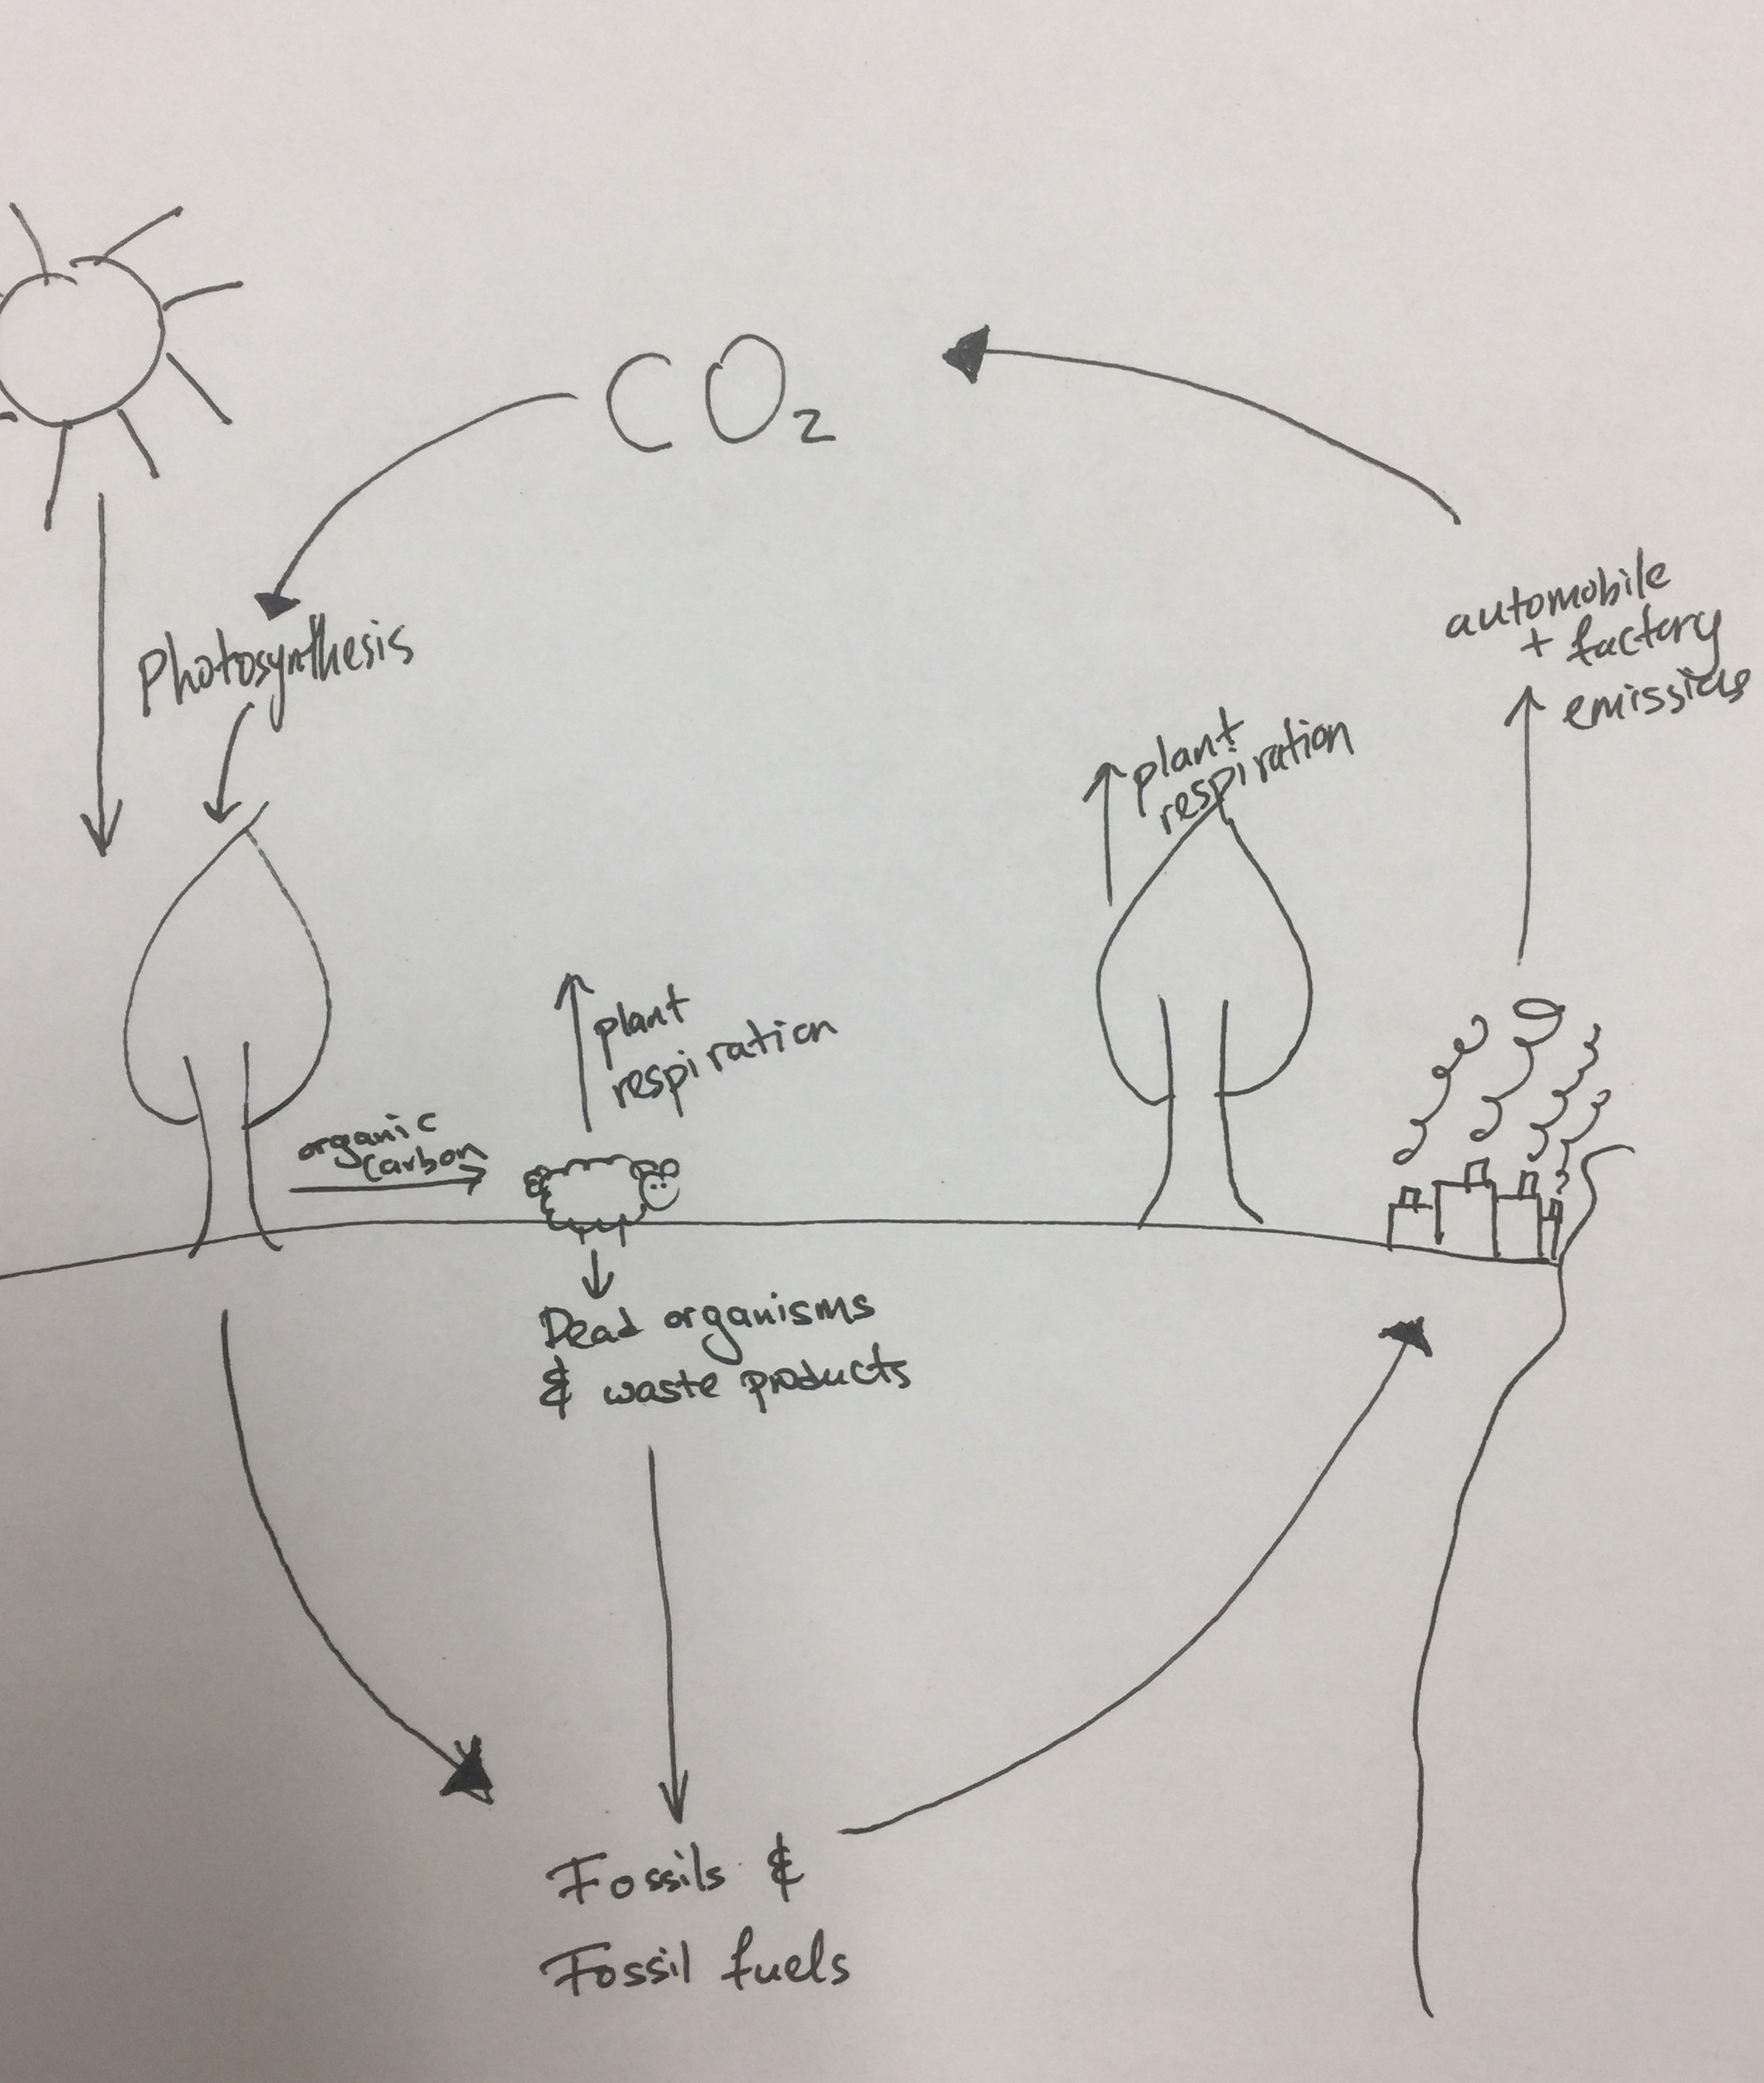
\includegraphics[width=\textwidth]{carboncycle}
\caption{The Carbon Cycle}
\label{fig:carbon cycle}
\end{figure}

Anthropogenic interference in the carbon cycle, for which you may find review in Figure \ref{fig:carboncycle}), has mostly come in the form of fossil fuel exploitation and land use change. When undisturbed land converts to agricultural land, we observe reduced carbon inputs into the soil and accelerated decomposition of soil organic carbon (SOC) \citep{van2007impact}. SOC is removed by erosion and deposited in environments that become to be known as depositional areas. Carbon flux between the soil and the atmosphere can occur through three different mechanisms: 

\begin{enumerate}
  \item Replacement of SOC from plant input atat sites experiencing erosion and decline in SOC for decomposition
  \item Deep burial of carbon and thereafter hindered decomposition
  \item Rise in the decomposition of SOC when the soil breaks down as it detaches or transports
\end{enumerate}

\subsection{Carbon Sinks and Sources}

\subsubsection{Agriculture and Carbon Storage}

A major contributor to the shift in carbon storage influxes in Southeast Asia continues to be the need for more agricultural land to provide to the growing population and economic growth. The countries in these region will suffer the worst soil degradation because of their tropical aspect \citep{scherr1999soil}. The agricultural systems of Southeast Asia is one of the major causes of carbon fluxes imbalances. The most intensive agricultural system Southeast Asia is the lowland rice farming systems that cover 197 million hectares of land \citep{dixon2001nonalcoholic}. The rice systems are heavily irrigated systems that produce two to three times a year \citep{cassman1995extrapolating}. The lowland rice paddies depend on N fertilizer for yield. The subsidiary corps from these systems can be seen to be oilseeds, maize, root crops, soybeans, sugarcane, cotton, vegetables and fruits in all areas.

\textit{Carbon in Mangroves} 

As mentioned earlier, Southeast Asia has some of the greatest potential to serve as a carbon sink in an industrializing world. This can be seen in one of the most prominent features of the region, mangrove forests. Mangrove forests grow in tropical and sub-tropical zones, residing at the intersections of freshwater, lands, and the ocean, usually found in brackish aquatic habitats \citep{bravo2017managing}. Considering their distribution across Southeast Asia, which constitutes a third of global presence,  mangroves have ecological and economic value that should not be underestimated. For example, they are exploited for fish and shrimp farming by indigenous communities in Vietnam as well as plain timber usage. Their immense biomass alone should kickstart a discussion on their carbon sequestration capabilities.

Mangroves can play a critical role in mitigating nutrient runoff to coastal regions, which is how they are usually framed in climate change discourse. We need to add their contribution to the carbon cycle in this context. The carbon cycle is present in terrestrial and oceanic spaces and in the transition between the two. Marine sediments and organic carbon found in mangroves can speak to the carbon sequestration potential of the ecosystem.

When mangroves shed dead material, this organic material does not thoroughly decompose, but instead the carbon can be converted to fossil fuel (compression of raw humus and creation of peat). Methane emissions from mangroves is of primary concern. It has been found that salinity and sulphate inhibit methane production by engaging sulphate-reducing bacteria which compete with methanogens. It has also been discovered that temperatures between 25 degrees celsius and 30 degrees celsius are optimal for methane emissions from the subsurface to the atmosphere. 

Moving forward, land use changes must be rethought and redeveloped. Mangroves experience their harshest degradation from direct human activity. To maintain their capabilities and capacities in nutrient cycling, reforestation and sustainable management policies must go into effect. First, though, it is also important for scientists to capture data on carbon storage in mangroves more accurately.

\textit{Borneo's Biomass} \newline
Let us dive into another case study in Borneo's forests, which are shared between two Southeast Asian nations, Indonesia and Malaysia. Borneo's forests are some of the most expansive in the region and are dominated by a single tree family known as Dipterocarpaceae \citep{qie2017long}. Unlike the Amazon and Congo Basin, Borneo's carbon-dense trees have not been treated with robust research on long-term biomass balance. Thus, it has been somewhat unclear in what ways Borneo's forests act as carbon sinks and sources.

What is known is that Borneo's forests are also one of the most fragmented in the world. This introduces edge effects which hinder biomass accumulation -- some studies have shown that the negative effects are even visible 400m deep from the edges. Another severe limiting factor for these forests in their ability to serve as sinks is extreme drought events, driven by El Nino for instance. As with rainfall, droughts are becoming more intense and frequent. 

The problem we face is that there has not been sufficient formal research conducted on the stress climate change causes, and this unequivocally raises the urgency to focus on Borneo. And, at first, the possibilities seem endless: could it be that CO2 inflates the biomass of trees? Or could it be that droughts are killing trees? Does net carbon source reduce because of edge effects from fragmentation? These questions are globalized, but nuances appear in different regions. Even if all are true, how do they compete in determine the ultimaate reduction or rise in carbon sequestration?

This particular study found that extreme drought events probably do not reverse long-term biomass accumulation because they are too short. The researchers estimated that a forest, on average, must maintain about 302 hectares to remain a carbon sink, depending on its shape and how penetrative edge effects are. Edges can decrease above-ground productivity and lead to biomass mortality. It seems that if edges are managed with healthy buffer zones, forests of almost any size can sustain themselves as carbon sinks because biomass along boundaries can survive. Still, large forest reserves are needed for preserving biodiversity.

\subsection{Soil Organic Carbon and Soil Erosion}

As a result of agricultural erosion, large amounts of SOC and sediments are transported laterally over the Earth. There are about three steps in soil erosion: mobilization, transportation, and deposition \citep{quinton2010impact}. Eroded land exposes subsurface soil which eventually can be transported to cover what is known as topsoil. This is why research that is exclusively performed on the topsoil can bring up questionable interpretations. 

Quantifying these aforementioned fluxes is not difficult, but climate change and land use are also dynamic processes, so relying on today's calculations may not help us predict future disturbances \citep{heimann2008terrestrial}.

From a meta-analysis conducted on tropical landuse change, we find that conversion to cropland, specifically perennial crops, reduces SOC most, by about 25\% to 30\% \citep{don2011impact}. Conversion to grassland is at 12\% and secondary forest is 9\%. If cropland is afforested, on average, it can gain 29\% in SOC. Hence, agricultural cultivation can alter carbon cycling. Still, modeling such a large system can be difficult.
Interestingly, erosion over land which results in mineralization, a process by which nutrients are rendered accessible to plants, tends to be relatively unimportant because carbon inventory does not correlate well with mineralization--even though SOC transported to rivers tends to result in substantial mineralization \citep{cole2007plumbing}. 

Also, it should be noted that erosion can actually lead to both release and sequestration of carbon. When soil is disturbed, it may immediately release carbon \citep{berhe2007significance}. Sometimes, erosion means that the subsoil mixes as the new topsoil, and if it binds organic matter then we may observe intake \citep{harden1999dynamic}. The latter depends on lower rates of SOC decomposition.

\subsection{Preview: Other Nutrient Cycles}
As the main reservoirs of nutrients, soils also have an impact on the phosphorus and nitrogen cycle, which we will attempt to infuse here to capture the relationship between erosion and biogeochemical cycles. Usually these two cycles are associated with aquatic impacts, but it is crucial to open up the discourse to terrestrial environment \citep{van2007impact}. When mineralization of soil carbon occurs, so does an increase in dissolved nitrogen and phosphorous due to soil mobilization \citep{jacinthe2002carbon}. Burial of carbon can lead to the stabilization of nitrogen as seen in the consistent Carbon-Nitrogen ratios in topsoils across a given ecosystem. Nitrogen cycling can also affect carbon cycling with biomass production \citep{van2006element}. If nitrogen is a limiting factor for biomass, then nitrogen can also be viewed as a limiting factor for carbon.





\subsection{Swidden and Fallow Cultivation practices}

Swiddening, the slashing and burning of forest is an age old practice widespread in Southeast Asian countries for agricultural production. The practice is linked to many rising environmental issues in the region. The transformation that swiddening those to the land through deforestation and decomposition effects are not fully understood and need to be further researched. Going hand in hand with Swiddening is fallowing, leaving the land plowed and exposed unseeded for a few growing seasons, is steadily decreasing. The decrease in fallowing systems is leading to the system being replaced by perennial crops like rubber, fruit trees, oil palm, and timber \citep{schmidt2009assessment}. Swiddening cultivation is a effective natural resource management that requires field rotation not crop rotation relying on the fallowing to sustain the crop production. Swiddening is found in sloping upland of the systems known for being environmentally destructive contributing to erosion, negative nutrient balances and CO2 emissions \citep{de2008soil}. Swiddening cultivation has also been seen beneficial in other studies towards providing hydrology, biodiversity, and carbon storage in soil and vegetation {powell20153}. The transformation consequence of swidden cultivation on carbon emission is its contribution to 20\% of global human carbon emissions \citep{meehl2007global}.

Carbon emission begin to rise when the change of pool SOC in aboveground biomass due to land charge. The tropical lowland forest have some of the highest aboveground carbon stocks of any vegetation in the world. In Southeast Asia carbon stocks in forest have a range of 254 to 647 Mg C ha$^{-1}$. SOC serves as nutrient pool, cation exchange pool and buffer against acidity and aluminium toxicity \citep{silver2000potential}.

\subsection{Peatlands}

Peatland are wetlands that are dominated by peat forming plants that originate from biological processes. Peatland make up 3\% of the earth and are mostly found in East Asia, Southeast Asia, the Caribbean and Central America, South America and southern Africa \citep{strack2008peatlands}. Peatland globally have a  significant role in storage of soil carbon. 

Forest tropical peatlands in Southeast Asia store 42,000 million metric tonnes (Mt) of soil carbon. The stability of this pool is at risk due to the recent decades of deforestation, drainage, and fire. 

Peatland are vital when it comes to biological process because of the immense amount of carbon storage you can find in the systems, carbon dioxide sink, and atmospheric methane point. Peatland contribute small portion to the emission of CH4  and N2O but the sequestration of CO2 are far greater \citep{strack2008peatlands}. The Greenhouse gases properties of peatland is a shifting role that depends on the peatlands ecology, hydrology, climate, and climate change. The CO2 emission at times can be so great that the peatland can change from a sink to a source at times. Changing vegetation can contribute to shifts in carbon sequestration due to elevated water and production.

The major actors to disturbing Peatlands natural processes  are agriculture, forestry, peat fuel extraction, and horticulture.  Indonesia 3.7 million hectares of peatland are drained and being used for agriculture. This dramatically decrease C fixation capacity and threatened greenhouse gas emissions

Peatland can serve a very powerful asset to assuring carbon sequestration and mitigate emissions in the region.

Three components have been found to contribute in the change of carbon flux between soil and atmosphere

\subsection {Carbon Emissions from Soils}



\subsection {Mapping of Emissions through Southeast Asia}
- Work for a later date -

\section{Takeaways}
[To fit with thesis: When it comes to pedogensis and carbon, Southeast Asia is a unique, releavant, and introguing region. While there are many subtopics within these fields, it seems like the interaction with water is one of the most important. As other chapters discuss sea level rise, dive deeper into mangroves, peatlands, and geologic hazards, we find that water interfaces is a recurring theme. Even before major anthropogenic expansion and interference in the soil, rainfall, rivers, and the formation of islands demonstrated the power of hydrology to transport and bury soils. As Southeast Asia capitalizes on farming, water continues to play a critical role. In this way we can observe that hydrology places man and nature in one scope, going against a prevailing grain that humans are separated from nature.]
